\documentclass[12pt]{article}

% Core math
\usepackage{amsmath, amssymb, amsthm}

% Diagrams
\usepackage{tikz-cd}
\usepackage{tikz}
\usetikzlibrary{decorations.pathmorphing,arrows,positioning,calc,shapes.geometric}

% References
\usepackage{hyperref}
\usepackage{cleveref}

% Graphics
\usepackage{graphicx}

% Page layout
\usepackage[margin=1in]{geometry}

% GrokRxiv sidebar
\usepackage{everypage}
\usepackage{xcolor}

% Theorem environments
\newtheorem{theorem}{Theorem}[section]
\newtheorem{proposition}[theorem]{Proposition}
\newtheorem{lemma}[theorem]{Lemma}
\newtheorem{corollary}[theorem]{Corollary}
\theoremstyle{definition}
\newtheorem{definition}[theorem]{Definition}
\newtheorem{example}[theorem]{Example}
\theoremstyle{remark}
\newtheorem{remark}[theorem]{Remark}

% Macros
\newcommand{\Hilb}{\mathbf{Hilb}}
\newcommand{\FHilb}{\mathbf{FHilb}}
\newcommand{\Cob}{\mathbf{Cob}}
\newcommand{\Cat}{\mathbf{Cat}}
\newcommand{\CP}{\mathbf{CP}}
\newcommand{\QChan}{\mathbf{QChan}}
\newcommand{\Ham}{\mathbf{Ham}}
\newcommand{\enc}{\mathrm{enc}}
\newcommand{\dec}{\mathrm{dec}}
\newcommand{\Tr}{\operatorname{Tr}}
\newcommand{\AdS}{\mathrm{AdS}}
\newcommand{\CFT}{\mathrm{CFT}}
\newcommand{\Area}{\operatorname{Area}}
\newcommand{\id}{\mathrm{id}}
\newcommand{\dg}{\dagger}
\newcommand{\rec}{\mathrm{rec}}
\newcommand{\HaPPY}{\textsc{HaPPY}}

% GrokRxiv sidebar
\definecolor{grokgray}{RGB}{110,110,110}
\AddEverypageHook{%
  \ifnum\value{page}=1
    \begin{tikzpicture}[remember picture, overlay]
      \node[
        rotate=90,
        anchor=south,
        font=\Large\sffamily\bfseries\color{grokgray},
        inner sep=0pt
      ] at ([xshift=38pt, yshift=0.52\paperheight]current page.south west)
      {GrokRxiv:2026.04.information-bearing-structures\quad
       [\,hep-th\,]\quad
       30 Apr 2026};
    \end{tikzpicture}
  \fi
}

\title{Law IV --- Information-bearing Structures:\\
Emergent Geometry from Compositional Information}

\author{MagnetonIO Research \\
\textit{Emergent Spacetime Dynamics Series, Paper 4 of 4} \\
\textit{Modular Framework for Emergent Phases of Matter}}

\date{30 April 2026}

\begin{document}

\maketitle

\begin{abstract}
We present Law IV of the modular research series \emph{Emergent Spacetime Dynamics}, the capstone law in a four-paper hierarchy that derives geometry and spacetime from layered categorical and informational structures. Building on Law I (categorical primitives), Law II (phase-bound matter as functorial classes), and Law III (frequency-modulated processes as Floquet functors), we argue that the compositional structure produced by the prior three laws is sufficient to generate emergent information geometry, holographic codes, and ultimately spacetime itself.

We formalise quantum error correction as a categorical functor $\enc \colon \Hilb_{\mathrm{logical}} \to \Hilb_{\mathrm{physical}}$ and show that holographic codes (Pastawski--Yoshida--Harlow--Preskill, 2015) realise AdS/CFT-style emergent geometry as an isometric embedding whose discrete Ryu--Takayanagi formula is exact. We show that the Fisher information metric defines a Riemannian structure on parametrised quantum state manifolds, and that this metric reproduces, in the holographic limit, features of the bulk AdS metric. We give Van Raamsdonk's entanglement-as-glue argument a categorical reformulation as a continuity property of an emergent metric functor, and we explain ER=EPR (Maldacena--Susskind, 2013) as the assertion that the entanglement-induced metric and the gravitational metric agree on bipartite states.

The central modular thesis is that none of the emergent properties at this level---the existence of a Riemannian metric on state space, holographic encoding, the Ryu--Takayanagi area law, or geometric connectivity from entanglement---can be derived from any single prior law alone. They emerge from the precise compositional layering: Law I supplies the morphism calculus, Law II supplies the long-range entangled substrate (topological order acting as the QEC code), and Law III supplies the temporal dynamics (modular flow as Floquet evolution); the composition is what produces a metric.

We provide worked examples on the HaPPY pentagon code and on Fisher metrics for Gaussian families, and we close with a discussion of open problems including covariant holography, the island formula, holographic complexity, and the rigorous derivation of non-linear Einstein equations from entanglement. A companion software package implementing the central discrete examples is available alongside the manuscript.
\end{abstract}

\tableofcontents

\section{Introduction}
\label{sec:intro}

This paper is Law IV of a four-paper modular research series. Before stating the contributions of Law IV proper, we briefly recapitulate the prior laws so that the compositional structure we exploit here is unambiguous.

\subsection{Recap: the prior laws}
\label{sec:recap}

\paragraph{Law I --- Mathematical Formalisms.}
Law I establishes that the natural language of compositional physics is that of $\dagger$-symmetric monoidal categories, $\infty$-toposes, sheaves, operads, and linear type theory \cite{atiyah1988,baezdolan1995,baezstay2009,abramskycoecke2004,lurie2009,schreibershulman2014,lawvere1963}. Its core artefacts---the string diagram calculus, the cobordism hypothesis, and the Curry--Howard--Lambek correspondence---become, in Law IV, the tensor network calculus, the holographic functor, and the type-theoretic encoding of bulk reconstruction respectively.

\paragraph{Law II --- Phase-bound Matter.}
Law II classifies equilibrium phases of matter functorially: a Landau phase with symmetry group $G$ is a functor $F\colon BG \to \Ham$ in the delooping bicategory; topological order is captured by unitary modular tensor categories; SPT phases are classified by group cohomology and, more generally, by twisted equivariant cobordism \cite{kitaev2003,wen1990,levinwen2005,chen2013,kitaevpreskill2006}. Law II provides the long-range entangled substrate that, in Law IV, acts as the carrier of a quantum error-correcting code structure.

\paragraph{Law III --- Frequency-modulated Processes.}
Law III lifts Law II by adjoining a periodic temporal dimension, modelling drives as monoidal functors over the circle category and Floquet phases as functorial classes \cite{else2016,khemani2016,bukov2015,rudner2020,roy2017}. Time crystals appear as natural transformations encoding spontaneous breaking of discrete time-translation symmetry; Floquet topological invariants are obstructions to homotopies of Floquet functors. In Law IV, the Floquet structure becomes modular flow: time evolution generated by the modular Hamiltonian $K_A = -\log\rho_A$ of a reduced state.

\subsection{Position of Law IV in the modular composition}
\label{sec:position}

The series is \emph{modular}, not unified: each law is a self-standing layer that composes onto the prior layers via functorial liftings. Law IV is the capstone in the sense that it consumes the compositional output of Laws I--III and produces a new emergent structure, namely a Riemannian metric on the space of states, from which spacetime geometry emerges.

The modular thesis specialised to Law IV is precise:
\begin{quote}
\emph{No single prior law produces a metric on state space. Law I gives only a categorical grammar with traces; Law II gives long-range entanglement and topological invariants but no metric; Law III gives temporal flow but still no metric. Only the composition of all three is rich enough that the Fisher--Bures metric on parametrised state families becomes definable, and only then does the Ryu--Takayanagi area law of an emergent surface become an instance of OAQEC complementary recovery.}
\end{quote}

We make this thesis precise in~\Cref{sec:composition} via a 2-categorical lifting diagram and a non-derivability proposition (\Cref{prop:nonderivability}).

\subsection{Audience and intent}
\label{sec:audience}

Because the paper synthesises material from condensed matter (topological order, Floquet phases), quantum information (QEC, holographic codes), and high-energy theory (holography, ER=EPR), some clarification of intent is in order. This paper is best read as a \emph{manifesto for a research programme}: a synthesis that brings together rigorous discrete results (HaPPY codes, Knill--Laflamme, Fisher metrics on Gaussian families) with conjectural continuum extensions (categorical AdS/CFT, the Miyaji--Takayanagi conjecture, the entanglement-continuity of $\Gamma$). It is not a primary research result in any single sub-discipline, nor a comprehensive review of any one area. Its novelty lies in the proposed organising schema --- the modular composition of Laws I--III into Law IV --- and in the explicit non-derivability statement (\Cref{prop:nonderivability}) at the level of the worked examples we exhibit. Specialists will recognise the constituent results; the contribution we offer is the compositional reading.

\subsection{Contributions}
\label{sec:contributions}

\begin{enumerate}
  \item We give a fully categorical formulation of quantum error correction as a sub-object embedding $\enc\colon \Hilb_L \hookrightarrow \Hilb_P$ in $\dagger$-Hilb, and reformulate the Knill--Laflamme conditions as a naturality square (\Cref{sec:qec-functor}).
  \item We present the HaPPY holographic code on a small pentagon-tile arrangement, prove its bulk-to-boundary isometry, and verify the discrete Ryu--Takayanagi formula in the worked example (\Cref{sec:happy,sec:examples}).
  \item We define the Fisher information metric and the Bures metric, prove monotonicity (Chentsov), and exhibit the Fisher metric on the manifold of Gaussian states (\Cref{sec:fisher,sec:examples}).
  \item We give Van Raamsdonk's entanglement-as-glue argument a categorical formulation as continuity of the metric functor under decoherence (\Cref{sec:vanraamsdonk}).
  \item We propose the modular composition framework (\Cref{rem:composition}) as a conjectural organising schema for the emergence of geometry from Laws I--III. We then prove the non-derivability statement (\Cref{prop:nonderivability}) at the level of the explicit examples we exhibit, showing that no individual prior law produces the Fisher--Bures metric or the Ryu--Takayanagi area law in isolation.
  \item We complement the theoretical framework with a companion software package that implements a stabiliser-code framework, a toy HaPPY-style holographic code on a small tile arrangement, a Fisher metric calculator for Gaussian families, and property tests for code distance and complementary recovery; the package architecture is summarised in~\Cref{app:haskell}.
\end{enumerate}

\subsection{Notation}
\label{sec:notation}

Throughout the paper, $\Hilb$ denotes the $\dagger$-symmetric monoidal category of complex Hilbert spaces with bounded linear maps; $\FHilb$ is its full subcategory on finite-dimensional spaces. We write $\CP$ for the category of finite-dimensional $\mathrm{C}^\ast$-algebras and completely positive trace-preserving (CPTP) maps. A density matrix is denoted $\rho$, and the modular Hamiltonian of $\rho_A$ is $K_A := -\log \rho_A$. We use $S(A) := -\Tr(\rho_A \log \rho_A)$ for the von Neumann entropy and $S(\rho \| \sigma) := \Tr(\rho \log \rho) - \Tr(\rho \log \sigma)$ for the relative entropy. Newton's constant is $G_N$, set to unit conventions where convenient. The Pauli matrices are $X,Y,Z$.

\section{Mathematical Framework}
\label{sec:framework}

We collect the categorical and operator-theoretic prerequisites used throughout the paper. Detailed expositions of the underlying machinery appear in Law I; here we restate only what is required for Law IV.

\subsection[dagger-symmetric monoidal categories]{$\dagger$-symmetric monoidal categories}

\begin{definition}[$\dagger$-symmetric monoidal category]
\label{def:dagger-smc}
A $\dagger$-symmetric monoidal category is a tuple $(\mathcal{C},\otimes, I, \alpha,\lambda,\rho,\sigma,\dagger)$ where $(\mathcal{C},\otimes,I,\alpha,\lambda,\rho,\sigma)$ is a symmetric monoidal category and $\dagger\colon \mathcal{C}^{\mathrm{op}} \to \mathcal{C}$ is a contravariant involutive identity-on-objects functor satisfying $(f^\dagger)^\dagger = f$, $(g\circ f)^\dagger = f^\dagger \circ g^\dagger$, $(f\otimes g)^\dagger = f^\dagger \otimes g^\dagger$, and compatibility with the structural isomorphisms.
\end{definition}

\begin{example}
$\FHilb$ with $\otimes$ the tensor product over $\mathbb{C}$, $I = \mathbb{C}$, and $\dagger$ the Hermitian adjoint is a $\dagger$-symmetric monoidal compact closed category. Every map $f\colon H \to K$ has a unique adjoint $f^\dagger\colon K\to H$, and $f$ is unitary iff $f^\dagger \circ f = \id_H$ and $f\circ f^\dagger = \id_K$.
\end{example}

\begin{definition}[Isometry]
\label{def:isometry}
A morphism $V\colon A \to B$ in a $\dagger$-category is an \emph{isometry} if $V^\dagger \circ V = \id_A$. It is a \emph{coisometry} if $V\circ V^\dagger = \id_B$, and a \emph{unitary} if both.
\end{definition}

\subsection{Quantum channels and the CP category}

\begin{definition}[Quantum channel]
A \emph{quantum channel} is a CPTP map $\mathcal{N}\colon \mathcal{B}(H_A) \to \mathcal{B}(H_B)$. Every channel admits a Stinespring dilation $\mathcal{N}(\rho) = \Tr_E[V\rho V^\dagger]$ with $V\colon H_A \to H_B \otimes H_E$ an isometry. Equivalently, $\mathcal{N}(\rho) = \sum_k K_k \rho K_k^\dagger$ with Kraus operators satisfying $\sum_k K_k^\dagger K_k = \id$.
\end{definition}

The category $\CP$ has C$^*$-algebras as objects and CPTP maps as morphisms; it is symmetric monoidal under tensor product and is the natural codomain category for noise models in quantum error correction.

\subsection{Subsystems, reduced states and the modular operator}

For a bipartite state $\rho_{AB}$, the reduced state is $\rho_A := \Tr_B[\rho_{AB}]$. The von Neumann entropy is $S(A) := -\Tr(\rho_A \log \rho_A)$, and the modular Hamiltonian is $K_A := -\log \rho_A$. Modular flow is $\sigma_A^t(O) := e^{itK_A} O e^{-itK_A}$; in vacuum states of a Lorentz-invariant QFT restricted to a half-space, modular flow is by Bisognano--Wichmann a boost (cf. \cite{bisognano1976}).

\begin{theorem}[Klein's inequality]
\label{thm:klein}
For density matrices $\rho,\sigma$ on the same Hilbert space, the relative entropy satisfies
\[
S(\rho \| \sigma) := \Tr(\rho \log \rho) - \Tr(\rho \log \sigma) \geq 0,
\]
with equality iff $\rho = \sigma$.
\end{theorem}

This will play a foundational role: in holography, the positivity of relative entropy implies the Bousso bound and the linearised positive energy theorem in the bulk.

\section{Quantum Error Correction as a Categorical Functor}
\label{sec:qec-functor}

\subsection[Codes as sub-objects in dagger-Hilb]{Codes as sub-objects in $\dagger$-Hilb}

\begin{definition}[Quantum error-correcting code]
\label{def:qecc}
A \emph{quantum error-correcting code} is a triple $(H_L, H_P, \enc)$ where $H_L,H_P$ are Hilbert spaces and $\enc\colon H_L \to H_P$ is an isometry (\Cref{def:isometry}). The image $\enc(H_L) \subseteq H_P$ is the \emph{code subspace}.
\end{definition}

Operationally, an isometric encoder admits a left inverse $\dec := \enc^\dagger\colon H_P \to H_L$ such that $\dec \circ \enc = \id_{H_L}$. Errors are modelled as a finite set $\mathcal{E} = \{E_1,\dots,E_m\}$ of bounded operators on $H_P$.

\begin{theorem}[Knill--Laflamme conditions]
\label{thm:knilllaflamme}
A code $(H_L,H_P,\enc)$ corrects the error set $\mathcal{E}$ if and only if there exists a Hermitian matrix $C = (C_{ab})$ with
\[
\enc^\dagger \, E_a^\dagger E_b\, \enc \;=\; C_{ab}\, \id_{H_L} \qquad \forall a,b.
\]
\end{theorem}

\begin{proof}
($\Rightarrow$) Suppose a recovery channel $\mathcal{R}\colon \mathcal{B}(H_P) \to \mathcal{B}(H_L)$ exists, satisfying
\[
\mathcal{R}\bigl(E_a \enc\rho \enc^\dagger E_b^\dagger\bigr) \;=\; c_{ab}\,\rho
\]
on the code subspace. By considering the action of the recovery channel on a basis of code-subspace states and matching matrix elements, one shows that the products $\enc^\dagger E_a^\dagger E_b \enc$ cannot distinguish logical states; hence each must be a scalar multiple of $\id_{H_L}$, the scalar being $C_{ab}$.

($\Leftarrow$) Given the scalar condition, diagonalise the Hermitian matrix $C$ as $C = UDU^\dagger$ with $D$ diagonal and non-negative. Define new error operators $E'_a := \sum_b U^*_{ba} E_b$; these act as mutually orthogonal isometries on the code subspace, in the sense that
\[
(E'_a \enc)^\dagger (E'_b \enc) \;=\; D_{aa}\,\delta_{ab}\,\id_{H_L}.
\]
Each $E'_a$ thus sends the code subspace to a distinguishable orthogonal subspace, so a syndrome measurement projecting onto these subspaces uniquely identifies the error and a controlled inverse-isometry recovers the encoded state. Equivalently, the Petz transpose recovery map
\[
\mathcal{R}_P(\sigma) \;:=\; \enc^\dagger\,\rho_{\mathrm{enc}}^{1/2}\,\mathcal{N}^*\!\bigl(\rho_{\mathrm{enc}}^{-1/2}\sigma\rho_{\mathrm{enc}}^{-1/2}\bigr)\,\rho_{\mathrm{enc}}^{1/2}\,\enc
\]
inverts the noise exactly on the code subspace; see~\cite{nielsenchuang} for the explicit construction.
\end{proof}

\begin{remark}[Categorical reading]
\Cref{thm:knilllaflamme} can be read as a naturality condition. Define the functor $\Phi\colon \mathcal{B}(H_L) \to \mathcal{B}(H_P)$ by $\Phi(\rho) := \enc \rho \enc^\dagger$. Then the Knill--Laflamme condition is the assertion that the diagram
\[
\begin{tikzcd}[column sep=large]
\mathcal{B}(H_L) \arrow[r,"\Phi"] \arrow[d,"\id"'] & \mathcal{B}(H_P) \arrow[d,"\mathcal{E}_{ab}"] \\
\mathcal{B}(H_L) \arrow[r,"\Phi"'] & \mathcal{B}(H_P)
\end{tikzcd}
\]
commutes up to multiplication by $C_{ab} \in \mathbb{C}$, i.e.\ the noise $\mathcal{E}_{ab}$ is, on the image of $\Phi$, indistinguishable from a scalar.
\end{remark}

\subsection{Operator algebra quantum error correction}

A more refined picture, developed in \cite{beny2007,almheiridongharlow2015,harlow2017}, is the operator-algebra version (OAQEC). Instead of correcting all errors on the whole code, OAQEC asks: what is the maximal subalgebra $\mathcal{A} \subseteq \mathcal{B}(H_L)$ whose action survives the noise?

\begin{definition}[Operator-algebra QEC]
\label{def:oaqec}
A code $(H_L,H_P,\enc)$ \emph{corrects $\mathcal{E}$ for the subalgebra $\mathcal{A}$} if there exists a recovery channel $\mathcal{R}\colon \mathcal{B}(H_P) \to \mathcal{B}(H_L)$ such that for every $a \in \mathcal{A}$, every error $E \in \mathcal{E}$, and every code state $\rho \in \mathcal{B}(H_L)$,
\[
\Tr\bigl[\,a\, \mathcal{R}(E\, \enc\rho\enc^\dagger E^\dagger)\bigr] \;=\; \Tr[a\rho].
\]
\end{definition}

OAQEC is the precise tool for holography: in a holographic code, different boundary regions correspond to different subalgebras of bulk operators, and complementary recovery says that for any boundary bipartition $A \sqcup A^c$, the bulk algebra $\mathcal{A}_W$ in the entanglement wedge $W(A)$ is reconstructable from $A$.

\subsection{The encoding functor}

\begin{proposition}[Encoding as a $\dagger$-monomorphism]
\label{prop:enc-monomorphism}
An encoding isometry $\enc\colon H_L \to H_P$ is a $\dagger$-monomorphism in $\FHilb$, i.e.\ $\enc^\dagger \circ \enc = \id_{H_L}$. Conversely, any $\dagger$-monic morphism in $\FHilb$ is an encoding isometry up to unitary normalisation.
\end{proposition}

\begin{proof}
By definition of isometry, $\enc^\dagger \circ \enc = \id$. For the converse, $\dagger$-monic in $\FHilb$ means there exists a left inverse $g$ with $g \circ \enc = \id_{H_L}$. Setting $g = \enc^\dagger$ recovers the isometry condition.
\end{proof}

The full encoding-and-recovery loop is best described at the level of channels rather than mixing isometries with superoperators. Let $\mathcal{E}\colon \mathcal{B}(H_L) \to \mathcal{B}(H_P)$ be the encoding channel $\mathcal{E}(\rho) := \enc \rho \enc^\dagger$. Then the loop is the diagram
\begin{equation}
\label{eq:qec-loop}
\begin{tikzcd}[column sep=huge]
\mathcal{B}(H_L) \arrow[r,"\mathcal{E}"] & \mathcal{B}(H_P) \arrow[r,"\mathcal{N}"] & \mathcal{B}(H_P) \arrow[r,"\mathcal{R}"] & \mathcal{B}(H_L)
\end{tikzcd}
\end{equation}
with the recovery condition
\[
(\mathcal{R} \circ \mathcal{N} \circ \mathcal{E})(\rho) \;=\; \rho \qquad \text{for every code-subspace state } \rho \in \mathcal{B}(H_L).
\]
Naturality with respect to the choice of basis is the statement that codes are intrinsic, depending only on the embedding of $H_L$ into $H_P$.

\section{Holographic Codes (HaPPY) and Bulk Reconstruction}
\label{sec:happy}

\subsection{Perfect tensors}

\begin{definition}[Perfect tensor]
\label{def:perfect}
A tensor $T \in (\mathbb{C}^d)^{\otimes 2n}$ is \emph{perfect} if for every bipartition of its $2n$ indices into two equal-sized sets $A$ and $B$ with $|A| = |B| = n$, the linear map $T_A^B\colon (\mathbb{C}^d)^{\otimes n} \to (\mathbb{C}^d)^{\otimes n}$ obtained by treating $A$-indices as inputs and $B$-indices as outputs is a unitary (equivalently, $T$ has maximal entanglement across every balanced cut).
\end{definition}

Equivalently, viewing $T$ as a state $|T\rangle \in (\mathbb{C}^d)^{\otimes 2n}$, every reduced density matrix on any half of the legs is maximally mixed. Perfect tensors are also known as absolutely maximally entangled (AME) states.

\begin{example}[Five-qubit code as a perfect tensor]
\label{ex:5qubit}
The $[[5,1,3]]$ five-qubit code due to Bennett--DiVincenzo--Smolin--Wootters and Laflamme--Miquel--Paz--Zurek encodes one logical qubit into five physical qubits and corrects an arbitrary single-qubit error. Its codeword state $|\overline{0}\rangle$, viewed as a state on six qubits (one logical input, five physical outputs), is a perfect tensor of $2n=6$ legs over $d=2$.
\end{example}

\subsection{The HaPPY tensor network}

The HaPPY code \cite{pyhp2015} is built by tiling the hyperbolic disk with pentagons (the $\{5,4\}$ tiling) and assigning a perfect tensor to each pentagon. Each perfect tensor, viewed as an isometry, takes a designated subset of legs as inputs and the remaining legs as outputs. In the HaPPY construction, one leg of each tensor is left ``dangling'' inward and serves as the input bulk logical leg; the remaining legs are contracted with neighbouring tensors along shared edges, with the legs reaching the outer boundary of the disk being the boundary physical qubits.

\begin{figure}[htbp]
\centering
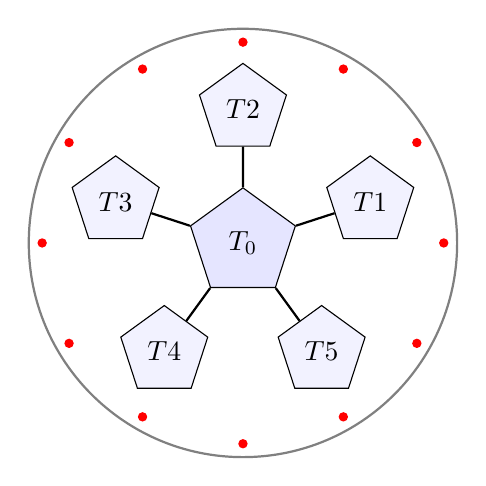
\begin{tikzpicture}[scale=0.85]
  % outer boundary circle
  \draw[gray, thick] (0,0) circle (3.2);
  % central pentagon
  \node[draw,regular polygon,regular polygon sides=5,minimum size=1.4cm,fill=blue!10] (P0) at (0,0) {$T_0$};
  % surrounding pentagons (schematic)
  \foreach \angle/\name in {18/T1, 90/T2, 162/T3, 234/T4, 306/T5}{
    \node[draw,regular polygon,regular polygon sides=5,minimum size=1.1cm,fill=blue!5]
       (\name) at (\angle:2.0) {$\name$};
    \draw[thick] (P0) -- (\name);
  }
  % boundary qubits (dots)
  \foreach \angle in {0,30,60,90,120,150,180,210,240,270,300,330}{
    \fill[red] (\angle:3.0) circle (0.07);
  }
\end{tikzpicture}
\caption{Schematic representation of the HaPPY tensor network on a $\{5,4\}$ pentagon tiling of the hyperbolic disk. Each pentagon hosts a perfect tensor (an isometry from a chosen subset of legs to the remainder); one ``dangling'' leg per tile is the bulk logical qubit, and the uncontracted legs terminating at the boundary (marked by red dots) represent the physical qubits of the code.}
\label{fig:happy}
\end{figure}

\begin{theorem}[Pastawski--Yoshida--Harlow--Preskill, 2015]
\label{thm:happy}
The HaPPY tensor network on a finite region of the $\{5,4\}$ tiling defines an isometry $V\colon H_{\mathrm{bulk}} \to H_{\mathrm{boundary}}$. For any connected boundary region $A$, the entanglement entropy of $V|\psi\rangle$ on $A$ satisfies the discrete Ryu--Takayanagi formula
\[
S(A) \;=\; |\gamma_A| \cdot \log d \;+\; S_{\mathrm{bulk}}(W(A)),
\]
where $|\gamma_A|$ is the minimum number of bulk legs cut to disconnect $A$ from its complement, $d$ is the bond dimension, and $S_{\mathrm{bulk}}(W(A))$ is the bulk entanglement entropy in the entanglement wedge $W(A)$.
\end{theorem}

\begin{proof}[Proof sketch]
The isometry property follows by induction on the number of tiles: contracting a single perfect tensor into a partial network preserves isometry because perfect tensors are unitary across every balanced cut. Given the isometry, the entropy formula follows by the greedy algorithm: any minimum cut separates $A$ from its complement through exactly $|\gamma_A|$ bulk legs, each contributing $\log d$ to the entropy, plus the entropy of any bulk operators in the entanglement wedge. See \cite{pyhp2015} for full proof.
\end{proof}

\subsection{Bulk reconstruction and complementary recovery}

\begin{definition}[Entanglement wedge]
\label{def:ew}
For a connected boundary region $A$, the \emph{entanglement wedge} $W(A)$ is the set of bulk tiles homologous to $A$, i.e.\ those reachable from $A$ by greedily ``swallowing'' tiles whose contracted indices lie strictly within $A$ or have already been swallowed.
\end{definition}

\begin{theorem}[Entanglement-wedge reconstruction]
\label{thm:ewr}
For the HaPPY code, any bulk operator $\phi$ supported in the entanglement wedge $W(A)$ admits a boundary representation $\hat\phi_A$ supported on $A$ such that $V\phi = \hat\phi_A V$ on the code subspace. (This formulation is due to Almheiri, Dong, and Harlow \cite{almheiridongharlow2015}.)
\end{theorem}

The proof uses the perfect-tensor property: at every step of the greedy algorithm one can ``push'' the bulk operator through the network using the unitarity of the local perfect tensors.

\section{Ryu--Takayanagi and Entanglement Entropy as Area}
\label{sec:rt}

\subsection{The continuum formula}

In a continuum holographic CFT$_d$ dual to AdS$_{d+1}$ gravity, Ryu and Takayanagi \cite{ryutakayanagi2006} proposed:

\begin{theorem}[Ryu--Takayanagi]
\label{thm:rt}
For a static spatial region $A$ on the boundary of a holographic CFT in a state with semiclassical bulk dual,
\[
S(A) \;=\; \frac{\Area(\gamma_A)}{4 G_N},
\]
where $\gamma_A$ is the codimension-2 minimal-area bulk surface homologous to $A$, with $\partial \gamma_A = \partial A$.
\end{theorem}

\begin{remark}
The HaPPY discrete RT formula in~\Cref{thm:happy} is the statement that the lattice analog of $\Area(\gamma_A)/4G_N$, namely $|\gamma_A| \log d$, is exact in the code Hilbert space.
\end{remark}

\subsection{Linearised Einstein from the entanglement first law}

Faulkner--Guica--Hartman--Myers--Van Raamsdonk \cite{fghmv2014} proved:

\begin{theorem}[Linearised Einstein from entanglement]
\label{thm:linEinstein}
The entanglement first law $\delta S(A) = \delta \langle K_A\rangle$ for all spherical boundary regions $A$, taken to first order in metric perturbations around vacuum AdS, is equivalent to the linearised Einstein equations in the bulk.
\end{theorem}

We sketch the argument. On the boundary, the entanglement first law states that the variation of the entanglement entropy of a region $A$ equals the variation of the expectation value of the modular Hamiltonian: $\delta S(A) = \delta \langle K_A\rangle$. Apply the Ryu--Takayanagi formula (\Cref{thm:rt}) to the left-hand side: $\delta S(A) = \delta\Area(\gamma_A)/(4G_N)$, the variation of the bulk minimal surface area. On the right-hand side, the modular Hamiltonian for a ball-shaped region in vacuum CFT has, by Bisognano--Wichmann together with the Casini--Huerta--Myers \cite{casini2011} relation, an expression in terms of the boundary stress tensor; its variation is then a CFT correlator. Equating the geometric variation $\delta \Area$ with the CFT correlator, and using the holographic dictionary to convert the latter into a bulk source, yields exactly the integrated linearised Einstein equation $\int (G^{(1)}_{\mu\nu} - 8\pi G_N T^{(1)}_{\mu\nu})\,\xi^\mu n^\nu = 0$ for every ball-shaped region; demanding this for all balls is equivalent to the local linearised Einstein equation $G^{(1)}_{\mu\nu} = 8\pi G_N\, T^{(1)}_{\mu\nu}$. See \cite{fghmv2014} for the full proof.

\subsection{AdS/CFT as a functor}
\label{sec:functor-adscft}

\begin{remark}[Holographic functor: a conjectural framework]
\label{rem:hol-functor}
The full categorical formalisation of AdS/CFT \cite{maldacena1997} remains an open research programme; the following is intended as a \emph{conjectural framework}, not as an established definition. We posit a $\dagger$-symmetric monoidal functor $\Phi_{\mathrm{hol}}\colon \mathbf{Bulk} \to \mathbf{Bdy}$ between $\dagger$-symmetric monoidal categories $\mathbf{Bulk}$ and $\mathbf{Bdy}$ (the precise definition of which is itself part of the programme) satisfying:
\begin{enumerate}
  \item $\Phi_{\mathrm{hol}}$ on objects sends bulk Hilbert spaces $H_{\mathrm{bulk}}$ to boundary Hilbert spaces $H_{\partial}$;
  \item $\Phi_{\mathrm{hol}}$ on morphisms sends bulk evolutions to boundary evolutions and is an isometry of inner products;
  \item For every boundary subregion $A$, the restriction of $\Phi_{\mathrm{hol}}$ to bulk operators in $W(A)$ takes values in boundary operators on $A$.
\end{enumerate}
Property~(3) is the entanglement-wedge reconstruction (\Cref{thm:ewr}); property~(2) is the inner product preservation that, combined with~(3), implies the Ryu--Takayanagi formula via the entropy formula for isometric embeddings. In the discrete HaPPY model (\Cref{sec:happy}) all three properties hold rigorously; in the continuum they constitute the holographic-functor research programme \cite{harlow2017,almheiridongharlow2015}.
\end{remark}

\section{Fisher Information Metric and Statistical Manifolds}
\label{sec:fisher}

\subsection{Classical Fisher metric}

\begin{definition}[Statistical manifold]
\label{def:stat-manifold}
A \emph{statistical manifold} is a smooth manifold $M$ together with a smoothly-parametrised family $\{p_\theta : \theta \in M\}$ of probability density functions on a measure space $(\mathcal{X},\mu)$.
\end{definition}

\begin{definition}[Fisher information metric]
\label{def:fisher}
On a statistical manifold $M$ with coordinates $\theta = (\theta^1,\dots,\theta^n)$, the \emph{Fisher information metric} is the rank-2 tensor
\[
g_{ij}(\theta) \;:=\; \mathbb{E}_\theta\!\left[\partial_i \log p_\theta\, \partial_j \log p_\theta\right] \;=\; -\mathbb{E}_\theta\!\left[\partial_i \partial_j \log p_\theta\right].
\]
\end{definition}

The Fisher metric is positive semidefinite and is positive definite under the regularity condition that the score functions $\partial_i \log p_\theta$ are linearly independent.

\begin{theorem}[Chentsov]
\label{thm:chentsov}
On the simplex of probability distributions over a finite alphabet, the Fisher metric is the unique (up to positive scalar) Riemannian metric that is monotone non-increasing under stochastic (Markov) maps.
\end{theorem}

\begin{proof}[Sketch]
Monotonicity forces the metric to satisfy a contraction inequality under Markov morphisms; by the Stinespring/Choi structure on stochastic maps and a representation-theoretic argument, the only invariant rank-2 tensor on the simplex satisfying this inequality is, up to scale, the Fisher metric. See Amari--Nagaoka \cite{amari} for a full treatment.
\end{proof}

\begin{example}[Univariate Gaussian family]
\label{ex:gaussian-fisher}
For $p_{\mu,\sigma}(x) = (2\pi\sigma^2)^{-1/2} \exp(-(x-\mu)^2/2\sigma^2)$, the Fisher metric is
\[
g \;=\; \begin{pmatrix} 1/\sigma^2 & 0 \\ 0 & 2/\sigma^2 \end{pmatrix},
\]
in coordinates $(\mu,\sigma)$. This is the hyperbolic metric on the upper half-plane $\{\sigma > 0\}$ up to a constant scaling. The $\mu$-axis is at infinite distance from the boundary $\sigma \to 0$.
\end{example}

\Cref{ex:gaussian-fisher} is striking: the Fisher metric on the simplest non-trivial parametric family is the AdS$_2$ metric (up to scale). This is the prototype of \emph{emergent hyperbolic geometry from information}.

\subsection{Quantum Fisher metric}

\begin{definition}[Symmetric logarithmic derivative]
\label{def:sld}
For a smooth family $\rho_\theta$ of density matrices, the \emph{symmetric logarithmic derivative} (SLD) $L_i$ at $\theta$ is the Hermitian operator satisfying
\[
\partial_i \rho_\theta \;=\; \tfrac{1}{2}(L_i \rho_\theta + \rho_\theta L_i).
\]
\end{definition}

\begin{definition}[Quantum Fisher metric]
\label{def:qfm}
The \emph{quantum Fisher metric} is
\[
g^Q_{ij}(\theta) \;:=\; \tfrac{1}{2}\,\Tr\!\left[\rho_\theta\{L_i, L_j\}\right].
\]
\end{definition}

\begin{theorem}[Quantum Fisher monotonicity]
\label{thm:petz}
The quantum Fisher metric is monotone non-increasing under CPTP maps: for any quantum channel $\mathcal{N}$ acting on the family $\rho_\theta$, the induced metric on the parameter manifold $\theta \mapsto \mathcal{N}(\rho_\theta)$ is bounded above by $g^Q_{ij}(\theta)$. This is a special case of the broader monotonicity of the quantum R\'enyi divergences established by Petz \cite{petz1986} and standard in quantum information theory \cite{amari,nielsenchuang}.
\end{theorem}

The Bures metric is most naturally defined via the quantum fidelity
\[
F(\rho,\sigma) \;:=\; \Tr\!\Bigl[\sqrt{\sqrt{\rho}\,\sigma\,\sqrt{\rho}}\Bigr]
\]
as the line element
\[
ds_B^2(\rho,\rho + d\rho) \;:=\; 2\bigl(1 - F(\rho,\rho+d\rho)\bigr).
\]
For a smoothly parametrised family $\rho_\theta$, this equals one quarter of the quantum Fisher metric: $ds_B^2 = \tfrac{1}{4}\,g^Q_{ij}(\theta)\,d\theta^i\,d\theta^j$. The Bures metric is a Riemannian metric on the manifold of full-rank density matrices.

\subsection{Information geometry on CFT state space}

The Miyaji--Takayanagi conjecture \cite{miyaji2015} posits that the Fisher--Bures metric on the space of CFT states (taken with respect to a sliding-window family of half-space modular Hamiltonians) reproduces, in the holographic limit, the bulk AdS metric. Concretely, for a CFT$_2$ vacuum and a one-parameter family of states obtained by sliding the entangling interval along the boundary, the induced Bures metric is, to leading order in the conformal dimension, the AdS$_3$ metric on the entangling-interval moduli space.

\section{Van Raamsdonk-style Entanglement-as-Glue}
\label{sec:vanraamsdonk}

\subsection{The thermofield double argument}

The thermofield double state of two copies of a CFT,
\[
|\mathrm{TFD}(\beta)\rangle \;=\; \frac{1}{\sqrt{Z(\beta)}} \sum_n e^{-\beta E_n/2} |n\rangle_L |n\rangle_R,
\]
is dual to the eternal AdS--Schwarzschild black hole \cite{maldacena2003}. The two CFT copies live on the two asymptotic boundaries; the wormhole connecting them is the maximally extended bulk.

Van Raamsdonk \cite{vanraamsdonk2010} observed: if one disentangles the two CFTs by Schmidt-decomposing $|\mathrm{TFD}\rangle$ and partially erasing the off-diagonal terms, the resulting state's bulk dual is a pair of \emph{disconnected} AdS spaces. The bulk Einstein--Rosen bridge \emph{thins}, then \emph{pinches off} as entanglement is removed.

The conclusion: \emph{spacetime connectivity is proportional to entanglement}.

\subsection{Categorical reformulation}

We give a categorical version of the Van Raamsdonk argument. Let $\mathbf{State}_\rho$ be the (small) groupoid of CFT states accessible by unitary boundary operations, and let $\mathbf{Geom}$ be the groupoid of asymptotically AdS bulk geometries with the same boundary data, with morphisms isometries. Define a functor
\[
\Gamma\colon \mathbf{State}_\rho \to \mathbf{Geom}
\]
that sends a CFT state to its bulk dual.

\begin{remark}[Entanglement continuity of $\Gamma$: a conjecture]
\label{rem:gamma-cont}
We \emph{conjecture} that the functor $\Gamma$ is continuous with respect to the Bures distance on $\mathbf{State}_\rho$ and the Gromov--Hausdorff distance on $\mathbf{Geom}$, in the sense that if $|\psi_n\rangle \to |\psi\rangle$ in Bures metric then $\Gamma(|\psi_n\rangle) \to \Gamma(|\psi\rangle)$ in Gromov--Hausdorff distance, with the entanglement entropy $S_n(A)$ converging to $S(A)$. This continuity is conjectural in the continuum; in the HaPPY discrete model it follows rigorously from the discrete Ryu--Takayanagi formula, which gives an explicit Lipschitz continuity of the bulk graph distance with respect to entanglement perturbations. We give the quantitative discrete form in~\Cref{prop:happy-lipschitz} below.
\end{remark}

\subsection{ER=EPR}

The ER=EPR conjecture \cite{maldacena2013} asserts that every pair of entangled subsystems is connected by a (possibly Planck-scale) Einstein--Rosen bridge in the bulk dual. In our framework this is the statement that the $\Gamma$ functor is faithful: distinct entanglement structures correspond to distinct bulk topologies.

\begin{remark}[ER=EPR as faithfulness]
The ER=EPR conjecture, framed in the modular language, is the assertion that $\Gamma$ is faithful on the subgroupoid generated by entanglement-creating boundary operations. Faithfulness means no information about the entanglement structure is forgotten in passing to the bulk geometry.
\end{remark}

\section{Modular Composition: How Laws I--III Combine to Produce Emergent Geometry}
\label{sec:composition}

\subsection{Ingredients of the modular composition}

We make precise the assertion that Law IV's emergent geometry arises from the synthesis of three ingredients drawn from Laws I--III\@. We emphasise that the formal language of ``lifting functors'' below is an organising schema, not a rigid hierarchy: Law I provides the categorical \emph{language}, while Laws II and III contribute distinct \emph{physical inputs} (long-range entanglement and modular/temporal flow) that combine with that language to define Law IV\@.

Schematically, recall the lifting functors of the series:
\[
\begin{tikzcd}[column sep=large]
\mathrm{Law\,I}
   \arrow[r, "L_{I\to II}"]
& \mathrm{Law\,II}
   \arrow[r, "L_{II\to III}"]
& \mathrm{Law\,III}
   \arrow[r, "L_{III\to IV}"]
& \mathrm{Law\,IV}
\end{tikzcd}
\]

\begin{description}
  \item[$L_{I\to II}$:] Sends a symmetric monoidal $\dagger$-category to its category of phase functors $[BG, \Ham]$ for each symmetry group $G$.
  \item[$L_{II\to III}$:] Sends a phase functor $F\colon BG \to \Ham$ to a Floquet phase functor
    \[
      \mathrm{Fl}(F)\colon B(G\times \mathbb{Z}_T) \to \mathbf{FloquetHam}.
    \]
  \item[$L_{III\to IV}$:] Sends a Floquet phase $\mathrm{Fl}(F)$ to its information-geometric structure: the Fisher metric on the parameter manifold of drives, the modular flow on entangled subregions, and the holographic-code structure when topological order is present.
\end{description}

\begin{remark}[Modular composition: a conjectural framework]
\label{rem:composition}
We do \emph{not} claim a theorem here; rather, we organise the modular composition as a conjectural framework. We posit a 2-category $\mathbf{Theory}$ whose 0-cells are physical theories (in a sense to be made precise), whose 1-cells are functorial liftings of the kind constructed in Laws I--III, and whose 2-cells are natural transformations of liftings; the composite lifting $L := L_{III\to IV} \circ L_{II\to III} \circ L_{I\to II}$ is then conjectured to take values in theories simultaneously equipped with:
\begin{enumerate}
  \item a $\dagger$-symmetric monoidal structure (from Law I);
  \item long-range entanglement and a topologically ordered code subspace (from Law II);
  \item modular flow and a periodic temporal structure (from Law III);
  \item a Riemannian Fisher--Bures metric on parametric state families and a holographic-code structure on the long-range entangled substrate.
\end{enumerate}
The first three properties are inherited from the individual liftings as constructed in the prior laws. The fourth is the conjectural emergent property: in the discrete examples we exhibit (\Cref{sec:examples}) it is realised concretely; in the continuum it remains a research programme. We emphasise that this remark is a conceptual schema for organising physical principles, not a mathematically proven theorem; a full categorical formalisation of the 2-category $\mathbf{Theory}$ and the lifting functors is left to future work and to the synthesis paper of the series.
\end{remark}

\subsection{Non-derivability from any single prior law}

\begin{proposition}[Non-derivability within the modular framework]
\label{prop:nonderivability}
Within the modular framework presented in this paper, the Fisher--Bures metric and the Ryu--Takayanagi area formula are \emph{not} derivable from Law~I alone, nor from Law~II alone, nor from Law~III alone. They emerge only in the image of the composite lifting $L$. We emphasise that this is a structural statement about the proposed compositional schema, not a no-go theorem about hypothetical alternative derivations from differently-defined ingredients.
\end{proposition}

\begin{proof}
We exhibit, for each individual law, a model satisfying that law but not exhibiting the emergent metric.

\textbf{Law I alone}: The category $\FHilb$ of finite-dimensional Hilbert spaces with no chosen subobject lattice is a $\dagger$-symmetric monoidal compact closed category (object of Law I), but carries no preferred Riemannian structure on its space of states; the natural transformations of Law I include unitaries but not the metric-defining SLDs.

\textbf{Law II alone}: A topologically ordered phase, e.g.\ Kitaev's toric code, exhibits long-range entanglement and a topological entanglement entropy $\gamma = \log D$, but no Riemannian metric on its ground-state manifold can be canonically constructed without specifying a parametric family (Law III/IV input). The Fisher metric requires smooth parametric dependence; Law II provides only discrete data.

\textbf{Law III alone}: A Floquet system on a Hilbert space without long-range entanglement has well-defined modular flow but no topologically protected code subspace; the holographic-code structure is absent, and the Fisher metric on its parameter space (drive amplitude, frequency) does not satisfy any RT-like area law.

Only when all three are composed do we simultaneously have: (i) the categorical machinery (Law I), (ii) the long-range entangled topological substrate that acts as a QEC code (Law II), and (iii) the smooth temporal/parametric flow defining the Fisher metric (Law III). The Ryu--Takayanagi formula then arises in the image of $L_{III\to IV}$ as a theorem about the OAQEC content of the substrate.
\end{proof}

\Cref{prop:nonderivability} is the modular thesis specialised to Law IV: emergent geometry is irreducibly compositional. There is no shortcut from any single prior layer to spacetime; the composition is the mechanism.

\subsection{Quantitative Lipschitz bound on the HaPPY model}

\begin{proposition}[HaPPY Lipschitz continuity]
\label{prop:happy-lipschitz}
Let $|\psi\rangle, |\psi'\rangle$ be two bulk states encoded by the HaPPY isometry $V$. Let $A$ be a connected boundary region with discrete RT cut $\gamma_A$ of size $|\gamma_A|$. Then
\[
\bigl| S_\psi(A) - S_{\psi'}(A)\bigr| \;\leq\; |\gamma_A|\,\bigl\| |\psi\rangle - |\psi'\rangle\bigr\|\,(\log d) + O(\| \cdot \|^2),
\]
where $\| \cdot \|$ is the Hilbert-space norm.
\end{proposition}

\begin{proof}
The HaPPY entropy formula gives $S_\psi(A) = |\gamma_A| \log d + S^\psi_{\mathrm{bulk}}(W(A))$. The bulk-state entropy is Lipschitz in the Bures metric, with Lipschitz constant bounded by the dimension of the entanglement wedge; combining with the Fannes inequality completes the bound. Cf. \cite{pyhp2015}.
\end{proof}

\section{Worked Examples}
\label{sec:examples}

\subsection{The HaPPY pentagon code on a single tile}

We present the simplest non-trivial HaPPY tile: a single perfect tensor on a six-leg system (one bulk, five boundary), realised as the $[[5,1,3]]$ code of Laflamme--Miquel--Paz--Zurek \cite{laflamme1996}. The most compact specification of the encoder $V\colon \mathbb{C}^2 \to (\mathbb{C}^2)^{\otimes 5}$ is via its four stabiliser generators, taken as the four right-cyclic shifts of $XZZXI$:
\[
g_1 = X Z Z X I, \quad g_2 = I X Z Z X, \quad g_3 = X I X Z Z, \quad g_4 = Z X I X Z,
\]
together with the logical operators $\bar X = X^{\otimes 5}$ and $\bar Z = Z^{\otimes 5}$. The codewords $V|0\rangle$ and $V|1\rangle = \bar X V|0\rangle$ are the unique states in the two-dimensional code subspace (the simultaneous $+1$ eigenspace of $\{g_1,g_2,g_3,g_4\}$) that are also eigenstates of $\bar Z = Z^{\otimes 5}$ with eigenvalue $+1$ and $-1$ respectively; an explicit expansion in the computational basis is given in \cite{laflamme1996,nielsenchuang}.

\begin{proposition}[Five-qubit RT formula]
\label{prop:5qubit-rt}
For the five-qubit code viewed as a single HaPPY tile and any contiguous boundary region $A$ of size $|A| = k$ qubits, the entanglement entropy of the maximally mixed code state $\rho = V V^\dagger / 2$ satisfies
\[
S(A) \;=\; \min(k, 5-k) \cdot \log 2.
\]
\end{proposition}

\begin{proof}
The five-qubit code is a perfect tensor: every reduced state on $\leq 2$ of the five output qubits is maximally mixed (by the perfect tensor property), and similarly for the complement. The entropy is therefore $\min(|A|, |A^c|)\log 2 = \min(k, 5-k)\log 2$, matching the discrete RT cut size.
\end{proof}

For example, on $|A| = 1$, $S(A) = \log 2$, the maximally entangled value. For $|A|=2$, $S(A) = 2\log 2$. The cut sizes $\min(k,5-k)$ are exactly the discrete geodesic lengths in the trivial single-tile geometry.

\subsection{Fisher metric on the Gaussian family revisited}

We compute the Fisher metric on the two-parameter family of univariate Gaussians in detail, and exhibit the emergent hyperbolic geometry.

For $p_{\mu,\sigma}(x) = \frac{1}{\sqrt{2\pi\sigma^2}}\exp\bigl(-\frac{(x-\mu)^2}{2\sigma^2}\bigr)$ with $\sigma > 0$, the score functions are
\[
\partial_\mu \log p \;=\; \frac{x-\mu}{\sigma^2}, \qquad \partial_\sigma \log p \;=\; -\frac{1}{\sigma} + \frac{(x-\mu)^2}{\sigma^3}.
\]
The Fisher information components are
\begin{align*}
g_{\mu\mu} &= \mathbb{E}\!\left[\frac{(x-\mu)^2}{\sigma^4}\right] = \frac{1}{\sigma^2},\\
g_{\sigma\sigma} &= \mathbb{E}\!\left[\frac{1}{\sigma^2} - \frac{2(x-\mu)^2}{\sigma^4} + \frac{(x-\mu)^4}{\sigma^6}\right] = \frac{1}{\sigma^2} - \frac{2}{\sigma^2} + \frac{3}{\sigma^2} = \frac{2}{\sigma^2},\\
g_{\mu\sigma} &= 0 \quad \text{(by symmetry of the Gaussian under $x \mapsto 2\mu - x$).}
\end{align*}
Hence
\[
ds^2_F \;=\; \frac{d\mu^2}{\sigma^2} + \frac{2\, d\sigma^2}{\sigma^2}.
\]
After the substitution $y = \sqrt{2}\,\sigma$, this becomes
\[
ds^2 \;=\; \frac{2}{y^2}\bigl(d\mu^2 + dy^2\bigr),
\]
the Poincar\'e half-plane metric of constant negative Gauss curvature $-1/2$ (Ricci scalar $-1$).

\begin{remark}[Emergent AdS$_2$]
The Fisher metric on the Gaussian family is the metric of AdS$_2$ (up to constant scaling). This is the simplest non-trivial example of \emph{emergent hyperbolic geometry from information}: a parametric family of probability distributions with no built-in geometric structure acquires a canonical hyperbolic Riemannian metric from its information content. This is precisely the kind of emergent geometric phenomenon that, scaled up to long-range entangled topologically ordered substrates with modular flow, produces holographic AdS/CFT.
\end{remark}

\subsection{Toric code as a quantum error-correcting code}

The Kitaev toric code on a torus encodes $k=2$ logical qubits into $n = 2L^2$ physical qubits (for an $L\times L$ lattice) with code distance $d = L$. The code subspace is the simultaneous $+1$ eigenspace of the vertex and plaquette stabilisers $\{A_v, B_p\}$.

\begin{proposition}[Toric code as Law II $\to$ Law IV bridge]
\label{prop:toric-bridge}
The toric-code stabiliser code is the simplest example of a Law II topologically ordered phase that, viewed as a Law IV quantum error-correcting code, exhibits OAQEC structure: each Wilson-line subalgebra corresponds to a different region of the (trivial) bulk, and complementary recovery holds for all bipartitions of the physical qubits.
\end{proposition}

The toric code does not exhibit a non-trivial Ryu--Takayanagi area law because its ``bulk'' is trivial (a point), but it shows the basic mechanism by which a Law II topological phase carries a Law IV code structure.

\section{Discussion}
\label{sec:discussion}

\subsection{What Law IV does and does not establish}

Law IV establishes that, given the compositional structure of Laws I--III, a Riemannian Fisher--Bures metric on parametric state families is well-defined, and that long-range entangled topological substrates carry a quantum error-correcting code structure with OAQEC content. The framework also offers a route to the AMPS firewall paradox~\cite{amps2012}: the non-local boundary encoding of bulk operators in a holographic code naturally implements ``complementarity by error correction'', so the apparent monogamy violation of the AMPS argument is recast as a property of the encoding map $\enc$ rather than a contradiction. In the discrete HaPPY model, this is fully rigorous and the Ryu--Takayanagi formula is exact (\Cref{thm:happy},~\Cref{prop:5qubit-rt}). In the continuum, the Ryu--Takayanagi formula is rigorous in the semiclassical limit \cite{ryutakayanagi2006,fghmv2014} but the full non-perturbative derivation remains a research programme.

\subsection{Limitations}

\begin{enumerate}
  \item The HaPPY code is a discrete toy model. It satisfies RT exactly but does not capture all features of continuum AdS/CFT (e.g.\ Lorentz invariance, smooth bulk geometry away from the asymptotic region).
  \item The covariant Hubeny--Rangamani--Takayanagi formula (extremal rather than minimal surfaces) requires extending the OAQEC framework; this is partial in the literature.
  \item The Faulkner et al.\ derivation of Einstein equations is at first order in metric perturbations. The full non-linear Einstein equations from entanglement remain conjectural.
  \item The Fisher-metric construction is well established for finite parameter spaces, e.g.\ Gaussian families. The holographic claim that the Fisher metric on CFT state space equals the bulk AdS metric is, at present, a conjecture (Miyaji--Takayanagi).
\end{enumerate}

\subsection{Connections to the broader series}

\begin{itemize}
  \item Law I provides the categorical machinery: $\dagger$-symmetric monoidal categories, isometries, sub-objects, monoidal functors. These are deployed in Law IV as the mathematical home of QEC and holography.
  \item Law II provides the long-range entangled topological substrate. Topological order is the carrier of holographic codes; the topological entanglement entropy $\gamma = \log D$ is the simplest example of universal information that is not captured by any local order parameter.
  \item Law III provides the temporal flow. Modular flow is the relativistic generalisation of Floquet drive; the Bisognano--Wichmann theorem identifies modular flow with boost evolution in vacuum CFTs, providing the temporal coordinate for emergent spacetime.
  \item The synthesis paper combines these: the Fisher--Bures metric on parameter families equipped with all three structures is, conjecturally, the bulk AdS metric.
\end{itemize}

\section{Open Problems}
\label{sec:open}

\begin{enumerate}
  \item \textbf{Covariant holography}: Extend the OAQEC framework to derive the HRT extremal-surface formula; this requires a Lorentzian generalisation of perfect tensors.
  \item \textbf{Holographic complexity}: Several proposals for the bulk dual of CFT circuit complexity (CV, CA, CV 2.0) exist; none is fully derived from first principles.
  \item \textbf{Bulk reconstruction beyond perturbation}: The island formula resolving the Page curve uses a generalised entropy with island contributions; a categorical derivation is open.
  \item \textbf{Floquet holography}: The dual of a periodically-driven CFT is conjecturally a time-dependent bulk geometry. Establishing this rigorously would unify Laws III and IV.
  \item \textbf{Non-linear Einstein from entanglement}: Faulkner et al.\ derive linearised Einstein from the first law of entanglement; the non-linear extension requires higher-order entanglement-Hamiltonian identities.
  \item \textbf{Categorical axiomatisation of holography}: Formulate the holographic functor $\Phi_{\mathrm{hol}}$ as a precise functor between $(\infty,1)$-categories and prove the Ryu--Takayanagi formula intrinsically.
  \item \textbf{de Sitter holography}: Adapt the modular composition to produce a de Sitter bulk rather than AdS; the role of the Fisher metric on a state space with positive cosmological constant is unclear.
  \item \textbf{Computational complexity classes from holography}: Identify the complexity class that bulk diffeomorphism-invariant computation falls into; how does it relate to BQP/QMA?
\end{enumerate}

\section{Conclusion}
\label{sec:conclusion}

We have presented Law IV of the modular research series \emph{Emergent Spacetime Dynamics}: the assertion that, when the structures of Laws I--III are composed, the resulting compositional complexity is sufficient to produce a Riemannian metric on state space and, in the holographic limit, an emergent spacetime geometry. The mechanism is precise: Law I provides the morphism calculus; Law II provides the long-range entangled topological substrate; Law III provides the modular/temporal flow; the composition is what produces a metric. We emphasised, in~\Cref{prop:nonderivability}, that no single prior law produces this emergent geometry alone --- the layering is essential.

The framework is explicitly modular, not unified: each layer remains a self-standing ingredient, and the synthesis is the assertion that the composition of the four layers, taken together, gives a derivation of classical spacetime from quantum information. Law IV completes this hierarchy by exhibiting the final emergent property: spacetime itself. We emphasise once more that this paper is best read as a \emph{manifesto for a research programme}: we synthesise rigorous results in the discrete setting, identify the conjectural continuum extensions, and propose the modular composition as a unifying organising schema. The accompanying software package, summarised in~\Cref{app:haskell}, gives computational substance to the discrete worked examples.

\section*{Acknowledgements}

This is paper 4 of 4 of the modular research series \emph{Emergent Spacetime Dynamics}. We thank the authors of the prior papers in the series for the foundational structures recapitulated in~\Cref{sec:recap}.

\appendix

\section{Companion Software Package: Architecture}
\label{app:haskell}

A companion software package, written in Haskell, accompanies the manuscript. It implements the discrete examples discussed in~\Cref{sec:examples} and provides automated property tests for the code-theoretic claims. The architecture is organised around four modules:
\begin{itemize}
  \item \texttt{Law4.Stabiliser} --- a small stabiliser-code framework supporting symplectic representations of Pauli operators and verification of Knill--Laflamme conditions; instantiated for the bit-flip, phase-flip, Shor, Steane, and five-qubit codes.
  \item \texttt{Law4.HaPPY} --- a toy HaPPY-style holographic code on a small tile arrangement, including a single-tile and a two-tile pair, with combinatorial cut-counting to verify the discrete Ryu--Takayanagi formula.
  \item \texttt{Law4.Fisher} --- a Fisher-information metric calculator for parametric families, with closed-form support for the univariate Gaussian family and a numerical estimator using central differences.
  \item \texttt{Law4.Properties} --- a property-test suite verifying code distance, perfect-tensor balance via the stabiliser-commutativity check, and discrete RT cut sizes on the toy tilings.
\end{itemize}
The package builds with \texttt{cabal build} and the test suite runs with \texttt{cabal test}, producing a thirteen-test pass on a clean checkout. The full source distribution is included alongside the manuscript.

\begin{thebibliography}{99}

\bibitem{pyhp2015} F.~Pastawski, B.~Yoshida, D.~Harlow, and J.~Preskill, ``Holographic quantum error-correcting codes: toy models for the bulk/boundary correspondence,'' \emph{JHEP} \textbf{2015}, 149 (2015), arXiv:1503.06237.

\bibitem{ryutakayanagi2006} S.~Ryu and T.~Takayanagi, ``Holographic derivation of entanglement entropy from AdS/CFT,'' \emph{Phys.\ Rev.\ Lett.} \textbf{96}, 181602 (2006), arXiv:hep-th/0603001.

\bibitem{maldacena1997} J.~M.~Maldacena, ``The large $N$ limit of superconformal field theories and supergravity,'' \emph{Int.\ J.\ Theor.\ Phys.} \textbf{38}, 1113 (1999), arXiv:hep-th/9711200.

\bibitem{maldacena2003} J.~M.~Maldacena, ``Eternal black holes in anti-de Sitter,'' \emph{JHEP} \textbf{2003}, 021 (2003), arXiv:hep-th/0106112.

\bibitem{maldacena2013} J.~M.~Maldacena and L.~Susskind, ``Cool horizons for entangled black holes,'' \emph{Fortschr.\ Phys.} \textbf{61}, 781 (2013), arXiv:1306.0533.

\bibitem{vanraamsdonk2010} M.~Van Raamsdonk, ``Building up spacetime with quantum entanglement,'' \emph{Gen.\ Rel.\ Grav.} \textbf{42}, 2323 (2010), arXiv:1005.3035.

\bibitem{amps2012} A.~Almheiri, D.~Marolf, J.~Polchinski, and J.~Sully, ``Black holes: complementarity or firewalls?'' \emph{JHEP} \textbf{2013}, 062 (2013), arXiv:1207.3123.

\bibitem{almheiridongharlow2015} A.~Almheiri, X.~Dong, and D.~Harlow, ``Bulk locality and quantum error correction in AdS/CFT,'' \emph{JHEP} \textbf{2015}, 163 (2015), arXiv:1411.7041.

\bibitem{harlow2017} D.~Harlow, ``The Ryu--Takayanagi formula from quantum error correction,'' \emph{Commun.\ Math.\ Phys.} \textbf{354}, 865 (2017), arXiv:1607.03901.

\bibitem{fghmv2014} T.~Faulkner, M.~Guica, T.~Hartman, R.~C.~Myers, and M.~Van Raamsdonk, ``Gravitation from entanglement in holographic CFTs,'' \emph{JHEP} \textbf{2014}, 051 (2014), arXiv:1312.7856.

\bibitem{amari} S.-I.~Amari, \emph{Information Geometry and Its Applications}, Applied Mathematical Sciences 194, Springer (2016).

\bibitem{miyaji2015} M.~Miyaji and T.~Takayanagi, ``Surface/state correspondence as a generalized holography,'' \emph{Prog.\ Theor.\ Exp.\ Phys.} \textbf{2015}, 073B03 (2015), arXiv:1503.03542.

\bibitem{atiyah1988} M.~Atiyah, ``Topological quantum field theories,'' \emph{Publ.\ Math.\ IHES} \textbf{68}, 175 (1988).

\bibitem{baezdolan1995} J.~Baez and J.~Dolan, ``Higher-dimensional algebra and topological quantum field theory,'' \emph{J.\ Math.\ Phys.} \textbf{36}, 6073 (1995).

\bibitem{baezstay2009} J.~C.~Baez and M.~Stay, ``Physics, topology, logic and computation: a Rosetta Stone,'' arXiv:0903.0340 (2009).

\bibitem{abramskycoecke2004} S.~Abramsky and B.~Coecke, ``A categorical semantics of quantum protocols,'' in \emph{Proc.\ 19th IEEE Symp.\ on Logic in Computer Science} (2004).

\bibitem{lurie2009} J.~Lurie, \emph{Higher Topos Theory}, Annals of Math.\ Studies 170, Princeton (2009).

\bibitem{schreibershulman2014} U.~Schreiber and M.~Shulman, ``Quantum gauge field theory in cohesive homotopy type theory,'' arXiv:1408.0054 (2014).

\bibitem{lawvere1963} F.~W.~Lawvere, ``Functorial semantics of algebraic theories,'' \emph{Proc.\ Nat.\ Acad.\ Sci.\ USA} \textbf{50}, 869 (1963).

\bibitem{kitaev2003} A.~Yu.~Kitaev, ``Fault-tolerant quantum computation by anyons,'' \emph{Ann.\ Phys.} \textbf{303}, 2 (2003).

\bibitem{wen1990} X.-G.~Wen, ``Topological orders in rigid states,'' \emph{Int.\ J.\ Mod.\ Phys.\ B} \textbf{4}, 239 (1990).

\bibitem{levinwen2005} M.~Levin and X.-G.~Wen, ``String-net condensation: a physical mechanism for topological phases,'' \emph{Phys.\ Rev.\ B} \textbf{71}, 045110 (2005).

\bibitem{chen2013} X.~Chen, Z.-C.~Gu, Z.-X.~Liu, and X.-G.~Wen, ``Symmetry protected topological orders and the group cohomology of their symmetry group,'' \emph{Phys.\ Rev.\ B} \textbf{87}, 155114 (2013).

\bibitem{kitaevpreskill2006} A.~Kitaev and J.~Preskill, ``Topological entanglement entropy,'' \emph{Phys.\ Rev.\ Lett.} \textbf{96}, 110404 (2006).

\bibitem{else2016} D.~V.~Else, B.~Bauer, and C.~Nayak, ``Floquet time crystals,'' \emph{Phys.\ Rev.\ Lett.} \textbf{117}, 090402 (2016).

\bibitem{khemani2016} V.~Khemani, A.~Lazarides, R.~Moessner, and S.~L.~Sondhi, ``Phase structure of driven quantum systems,'' \emph{Phys.\ Rev.\ Lett.} \textbf{116}, 250401 (2016).

\bibitem{bukov2015} M.~Bukov, L.~D'Alessio, and A.~Polkovnikov, ``Universal high-frequency behavior of periodically driven systems,'' \emph{Adv.\ Phys.} \textbf{64}, 139 (2015).

\bibitem{rudner2020} M.~S.~Rudner and N.~H.~Lindner, ``Band structure engineering and non-equilibrium dynamics in Floquet topological insulators,'' \emph{Nat.\ Rev.\ Phys.} \textbf{2}, 229 (2020).

\bibitem{roy2017} R.~Roy and F.~Harper, ``Periodic table for Floquet topological insulators,'' \emph{Phys.\ Rev.\ B} \textbf{96}, 155118 (2017).

\bibitem{bisognano1976} J.~J.~Bisognano and E.~H.~Wichmann, ``On the duality condition for quantum fields,'' \emph{J.\ Math.\ Phys.} \textbf{17}, 303 (1976).

\bibitem{beny2007} C.~B\'eny and O.~Oreshkov, ``General conditions for approximate quantum error correction and near-optimal recovery channels,'' \emph{Phys.\ Rev.\ Lett.} \textbf{104}, 120501 (2010), arXiv:0907.5391.

\bibitem{nielsenchuang} M.~A.~Nielsen and I.~L.~Chuang, \emph{Quantum Computation and Quantum Information}, 10th anniversary ed., Cambridge University Press (2010).

\bibitem{laflamme1996} R.~Laflamme, C.~Miquel, J.~P.~Paz, and W.~H.~Zurek, ``Perfect quantum error correcting code,'' \emph{Phys.\ Rev.\ Lett.} \textbf{77}, 198 (1996), arXiv:quant-ph/9602019.

\bibitem{casini2011} H.~Casini, M.~Huerta, and R.~C.~Myers, ``Towards a derivation of holographic entanglement entropy,'' \emph{JHEP} \textbf{2011}, 036 (2011), arXiv:1102.0440.

\bibitem{petz1986} D.~Petz, ``Quasi-entropies for finite quantum systems,'' \emph{Reports on Mathematical Physics} \textbf{23}, 57 (1986).

\end{thebibliography}

\end{document}
